%%%%%%%%%%%%%%%%%%%%%%%%%%%%%%%%%%%%%%%%%%%%%%%%%%
%
%  New template code for TAMU Theses and Dissertations starting Fall 2012.  
%  For more info about this template or the 
%  TAMU LaTeX User's Group, see http://www.howdy.me/.
%
%  Author: Wendy Lynn Turner 
%	 Version 1.0 
%  Last updated 8/5/2012
%
%%%%%%%%%%%%%%%%%%%%%%%%%%%%%%%%%%%%%%%%%%%%%%%%%%%
%%%%%%%%%%%%%%%%%%%%%%%%%%%%%%%%%%%%%%%%%%%%%%%%%%%%%%%%%%%%%%%%%%%%%%
%%                           SECTION IV
%%%%%%%%%%%%%%%%%%%%%%%%%%%%%%%%%%%%%%%%%%%%%%%%%%%%%%%%%%%%%%%%%%%%%

\chapter{\uppercase{Implementation of Seismic Analytics Cloud Platform}}
To solve the problems stated in pevious chapters, we develop seismic analytics cloud platform (SAC for short). The goal of SAC is to deliver a scalable and productive cloud Platform as a Service (PaaS) to seismic data analysis researchers and developers. SAC has two main characteristics: one is able to process big data and another is easy to use for geology domain experts. With SAC, user only need focus on data analytics logic itself without caring about details on data storage and computing model. 

%SAC is designed to be able to store large amount of seismic data with major vendor's formats, as well as be able to process them in the scalable fashion to meet the performance requirements. Users should be able to work on their seismic processing algorithms using high-level programming models with very limited knowledge in parallelism and architecture.

\section{Architecture of SAC}

In the beginning, the mainframe is widely used for seismic data processing and each job regardless of running time needs to be put into queue waiting for execution. With the improvement of CPU power, more softwares were transferred to personal computer(PC) for better portability and interactivity. But with the growth volume size of seismic data, frequency of single core could not increase limitless and scalable resources are need to handle variable requirements, more and more softwares are then moved to cloud platform by utilizing parallelization dynamically. Such trend brings big change on business model: from selling software license to charging for service. In cloud platform, the thin client could request storage and computation resources basing on requirement, and in such way whole cluster or huge data center could be used efficiently. In HPC domain, MPI or PVM could also build on cluster, which fully utilize all resources in whole cluster but need deep understanding of data distribution and communication. The data storage in HPC is typical using centralized storage manager with disk array, which needs data movement between storage nodes and worker nodes. To overcome problems of HPC, we build SAC as service with template-based programming interface on cloud platform, and to make it easy to use, some popular image processing and signal processing software packages are integrated into SAC.  


Figure \ref{SACSWStack} shows the overall software stack used in SAC. In this diagram, the operating systems at 1st level from bottom to top could be Unix-like or Windows system running on virtual machine or bare metal. Above the OS layer, there should be a layer provides compiling and running environment, which include JRE/JDK, Scala, Python and other native libraries such as OpenCV \cite{OpenCVMain}, FFTW \cite{Frigo05thedesign} etc. Java has already became the dominating language in application development for its cross-platform and simplicity \cite{Top10Lang}. Scala is a new general-purpose programming language that support both object\-oriented and functional programming language but still runs on JVM and is compatible with existing Java libraries. Most big data processing platform such as Hadoop, Storm, HBase and Cassandra etc. are written in Java and provide Java programming interfaces; Spark is developed in Scala itself but applications running on it could be developed in Java, Scala or Python. For the performance issue, some computation intense libraries such FFTW and OpenCV are written in C++, but they also provide Java interface through JNI that could be used on JVM. In third layer, there are some common componets installed including HDFS, Mesos \cite{ApacheMesos} and YARN \cite{ApacheHadoop}  used for data storage and resource scheduling. HDFS is distributed file system delivered in Hadoop that provides highly fault-tolerance and high throughput access to big data set. In SAC, HDFS is used for storing original binary seismic data. The metadata and intermediate data such as seismic attribute are stored in Cassandra database. Resource management in cluster is very important for job scheduling and load balance, and in SAC, Standalone, Mesos and YARN are all supported. In the fourth layer from bottom, it includes the actual computation components: signal and image processing libraries with Java/Scala interface; Breeze \cite{ScalaNLPBreeze} is a set of libraries for machine learning and numerical computing written in Scala and Java. FFTW is a C subroutine library for computing the discrete Fourier transform (DFT) with one or more dimensions in both real and complex data format. There are already some Java FFTW wrappers make it could be used on JVM without giving up performance. SAC chose Spark as computation platform due to its performance achieved with in\-memory computation and its fault tolerance. The main work of this paper are focus on second and third layer from top. Seismic Analytics Cloud layer is used for providing SDK and running environment for client applications.SAC Framework plays most important role in this cloud platform, and it is the bridge of user's application and running environment on cluster. Template-Based framework provides common programming models for domain specific experts, and workflow could connect piece of algorithms or models into a job chain as well as run it automatically. Visualization is important for user to view results and generate useful information intuitively. Seismic Applications on the top of stack are mainly developed by end users. There is a user friendly web interface provided to user, on which user could view datasets, programming and testing single algorithm or running workflow in convenient way by drag\-and\-drop of widgets. Some other issues should also be considered on cloud platform, such as data security, job scheduling and resource sharing etc.   

%The design of SAC architecture is to emphasize twofold: one is to provide a high-level productive programming interface to simplify the programming efforts; the other is to execute user's applications with scalable performance. To achieve the first goal, we provide the web interface in which user could manage seismic datasets, programming within a variety of templates, generate complete source codes, compiling and then running the application and monitoring the job running status in SAC. 

%The interface allows users to write seismic data processing algorithms using our extracted common seismic computation templates, which lets users focus on their kernel algorithm implementation, and simplifies user's implementation in handling seismic data distribution and parallelism. While the most popular-used programming models in seismic data processing include MATLAB, Python, C/C++, Fortran, Java and more, SAC supports Java, Python and Scala natively, so that users can write their own processing algorithms directly on our platform with these three languages; For legacy applications written in other languages, SAC uses the so-called PIPE mode to handle input and output data as standard-in and -out, which requires minor modifications of program source code on handling input and output. SAC will generate complete Spark codes based on user's kernel codes and configurations, and then launch and monitor it on the SAC environment. In order to support large amount data storage and scalable I/O performance, we chose Hadoop HDFS as the underlying file system, which provides fault tolerance with duplicated copies and good I/O throughput by supporting data locality information to applications. HDFS supplies out-of-the-box redundancy, failover capabilities, big data storage and portability. Since the size of seismic data is very large and keeps increasing constantly, HDFS provides a good solution for the data storage with fault tolerance property.

%We use Spark as the parallel execution engine to start applications, since Spark works well on top of HDFS, Mesos [13] and YARN, and it provides a big data analytics computing framework with both in-memory and fault-tolerance support. Spark provides RDD \cite{SparkRDD} as a distributed memory abstraction that lets programmers perform in-memory computations on large-scale cluster/cloud in a fault-tolerant manner. To get better performance, we need to put frequently used data into memory and processing data in memory, which is one key performance boost comparing with MapReduce.Some other useful packages and algorithms in data analytics, such as SQL, machine learning and graph processing, are also provided in Spark distribution version. We also integrated some common used libraries for image processing and signal processing, such as OpenCV, Breeze and FFTW etc., to provide a rich third party of libraries support to speed up the development process. Figure \ref{SACSWStack} shows the overall software stack used in SAC.

%Figure \ref{SACArch} presents the overall architecture of SAC. Based on the SAC web interface, Users are able to upload, view and manage their seismic data, which are stored on HDFS. They can then create their application projects by selecting a template from a list of predefined templates to start their own programming. After selected dataset and processing pattern, writing codes and compiling successfully, users can configure the running parameters and then submit jobs to SAC. Job status could be monitored while job is running and running results could be checked after job is finished. On the SAC backend, a big seismic data file will be split into multi-partitions and be constructed into RDD, which will be processed by working threads that apply user's algorithm in parallel. After all data are processed, the output data will be saved back to HDFS.

Figure \ref{SACArch} shows the overall architecture of SAC, in which there are three main parts: data flow, operations on data and user interface.
The upper part of such diagram shows a complete processing lifecycle of seismic data on SAC; At first, seismic data need to be uploaded to HDFS. In the view of end user, it is still a big file, but HDFS will store it on different nodes block by block. User could also preprocess and view data as needed. To make such a huge file be processed by multi\-nodes, it will be splitted into small partitions and then user's transformations could be applied on them. When all operations on each partition finished, user could run some actions to persist results. Such results could be used for further processing, visualization or statistics etc.  

%%%%%%%%%%%%%%%%%%%%%%%%%%%%%%%%%%%%%%%%%%%%%%%%%%%%%%
\begin{figure}[h]
\centering
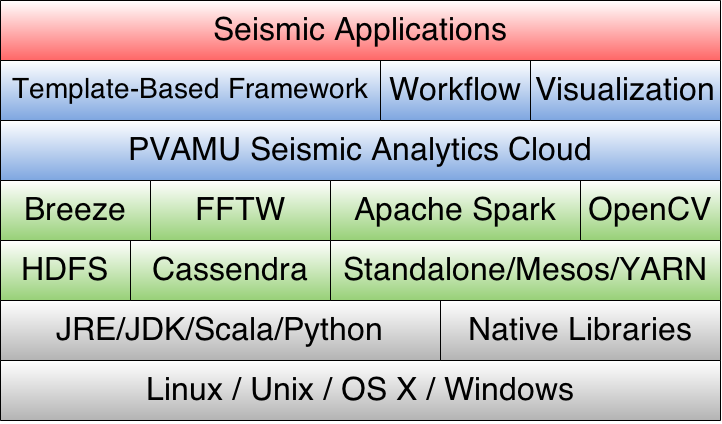
\includegraphics[scale=.50]{figures/SACSWStack.png}
\caption{The Software Stack of Seismic Analytics Cloud Platform}
\label{SACSWStack}
\end{figure}
%%%%%%%%%%%%%%%%%%%%%%%%%%%%%%%%%%%%%%%%%%%%%%%%%%%%%%

%%%%%%%%%%%%%%%%%%%%%%%%%%%%%%%%%%%%%%%%%%%%%%%%%%%%%%%
\begin{figure}[h]
\centering
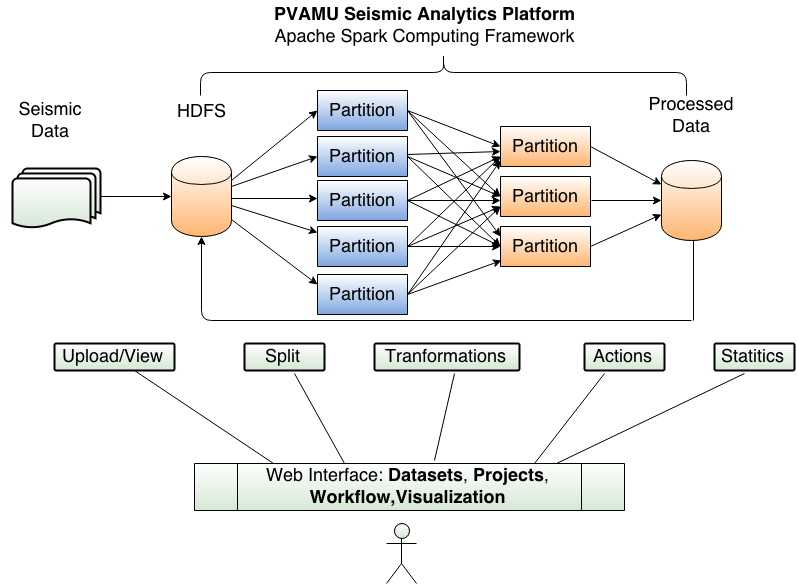
\includegraphics[scale=.50]{figures/SACArch.png}
\caption{The Architecture of Seismic Analytics Cloud Platform}
\label{SACArch}
\end{figure}
%%%%%%%%%%%%%%%%%%%%%%%%%%%%%%%%%%%%%%%%%%%%%%%%%%%%%%%

\section{Data Storage and Distribution}

There are many file formats used for storing seismic data, such as SEGY \cite{SEGYREV1}, SEGD \cite{SEGDREV21}, SEED \cite{IRISSEED} etc. Some popular softwares even have their own intermediate formats to make it easy for processing; Sesimic Unix has SU file format, OpendTect \cite{OpendTectMainPage} use CBVS(Common Binary Volume Storage) format, and SEPlib has its own SEP3D file format that seperate ASCII metadata with actual binary trace data. In current stage, only widely used SEGY file format is supported in SAC. Other data formats could be easily added in data preprocess stage.
The SEGY (also SEG-Y) \cite{SEGYREV1} file format is one of several standards developed by the Society of Exploration Geophysicists (SEG) for storing geophysical data. It consists of 3200 bytes textual file header, 400 bytes binary file header and trace data. Each trace has a 240 bytes header and variable binary trace data. In normal case, application need to parse file header to get some useful information about survey at first, then get a 2D/3D volume for further processing. To process SEGY file in parallel, such big seismic data needs to be split into multiple small partitions. The SEGY file could not be split directly: every worker node need to access header description information, and not all traces have same size of data. Meanwhile, most algorithms need to use one complete trace or plance as input, so one trace or one line could span more than two splits.   

So we introduce a preprocess program, transferring SEGY file into two files: one is xml file used to describe metadata, another file saves all traces data with equal size after interpolation. There are two pros with this format: xml file sharing same trace data file could save some other job related information about how to split trace data, and only xml files needs to be changed in most cases; trace data file could be split easily on requirement. Hadoop use InputFormat to split data, Which is also supported by Spark. The default InputFormat classes could not handle text file and binary file together, so we implemented a new SeismicInputFormat class in SAC. SeismicInputFormat use xml file as input, trying to parsing information from it and generate split list. Spark driver will send split to each executor, and then each task in executor will call SeismicRecordReader get trace data from file on HDFS. After Spark load seismic data from HDFS, it will generate an in-memory RDD for improving performance. The basic information about survey such as location of related trace data file, dimension, data type information are store in xml file, and beside those, user cloud also define other parameters used for application running. When user create a new project, he could define how many lines each split and number of overlap lines, and such parameters determine the offset and size of each split. As a rule, the seismic data is stored trace by trace in Inline direction, but there may be some algorithms need to process data in cross-line for time-depth direction. Such directon could also be defined in xml file, and SAC will load data in Inline direction into memory and then make in-memory transformation to generate a new direction RDD.
  
%However, SEGY data could not be split directly due to its irregularity, so we preprocess the SEG Y data format into a regular 3D volume data, and store the important header information into one xml file. Then the 3D volume data and xml will be feed into Spark applications. Spark uses InputFormat, which is the base class inherited from Hadoop to split such data and construct RDD. Each split will be mapped to one partition in RDD. The embedded InputFormat classes could not handle binary seismic data, so we implemented SeismicInputFormat in this project.  Based on configuration defined by user while creating project, such as how many lines each split and number of overlap lines, SeismicInputFormat could spilt the 3D volume and feed partition to each mapper. The data of 3D volume is stored trace by trace in the Inline direction by default. For some algorithms that need to process data in cross-line or time-depth direction, we also provide interfaces to transform Inline format RDD into cross-line or time-depth direction. In this way, we could cache Inline format RDD in memory, thus all the transformations could be executed in memory with better performance.

%\begin{table}[H]
%\centering
%\caption{This is a table template}
%\begin{tabular}{|l|c|c|c|c|c|}
%\hline
%Product & 1 & 2 & 3 & 4 & 5\\
%\hline
%Price & 124.- & 136.- & 85.- & 156.- & 23.-\\
%Guarantee [years] & 1 & 2 & - & 3 & 1\\
%Rating & 89\% & 84\% & 51\% & & 45\%\\
%\hline
%\hline
%Recommended & yes & yes & no & no & no\\
%\hline
%\end{tabular}
%\label{tab:template2}
%\end{table}

\section{Seismic RDD}
Resilient Distributed Datasets (RDDs) \cite{SparkRDD} is core concept proposed by Spark, which is a fault-tolerant collection of elements that can be operated on in parallel. RDDs \cite{ApacheSparkPG} support two types of operations: transformations, which create a new dataset from an existing one, and actions, which return a value to the driver program after running a computation on the dataset. Even in parallel programming on cluster, the programm still consists of data structure and algorithms. Spark uses the RDD as a common data structure that distributed in multi-nodes, and provides some typical operations as algorithm frameworks in functional language style so that user could plug in his own algorithms and apply them on RDD. Comparing with traditional parallel programming model such as MPI and OpenMP, the programming on Spark is much simpler. But for geophysicists or data scientists who have no much idea about RDD and functional language, there are still some tedious works to do. SAC tried to simplify work by introducing Seismic RDD and Template. User only need configure some parameters: The dataset need to process, input and output type of algorithms, then write a piece of codes, SAC will generate Seismic RDD, create template, merge user's codes and run them automatically. Seismic RDD is built from SeismicInputFormat, and besides the basic operations provided by Spark, Seismic RDD also provide some other features: fine-grain function on pixel or trace inside each split, transferring RDD from default inline direction to other directions automatically basing on configuration, override some operators for easily used by high level applications. The most advantage of RDD is caching most frequently used data in memory, thus improving performance of some iteration algorithms drastically. In normal case, the RDD is only valid within the lifetime of SparkContext, so RDD in memory will be discarded after application finished. Spark-jobserver \cite{SparkJobserver} provides a RESTful interface for submitting and managing Apache Spark jobs, jars, and job contexts, and moreover it introduces the concept of Named RDDs. With Named RDDs, serveral applications or jobs sharing the same context could cache and retrieve RDDs by name, thus improve RDD sharing and reuse among jobs. In workflow component of SAC, serveral jobs in one workflow will use Named RDDs to avoid loading and releasing RDD frequently in each job.

\section{Template}

%Based on the general parallel execution patterns of seismic processing algorithms and applications, we predefined some templates to make this framework easy to program. Every template has explicit input type and output type. The typical templates are: Pixel pattern, which use sub-volume or one pixel as input and output one pixel; Line pattern, which treat one line as input and one line as output; SubVolume pattern, which feed user’s application with sub-volume and get output from it in sub-volume format. A high level SeismicVolume class has been implemented in this project to provide user interface to access seismic volume. SeismicVolume class provides functions for constructing RDD based on processing templates user had selected, applying user's algorithms on RDD, and storing the final RDD on HDFS with format defined by user. To make it easy for programming, we provide some other functions to change the linear array into 2D matrix and 3D volume class; some functional programming interface such as iteration, map/flatMap, filter and zip could be used. We also integrated commonly used high-level algorithms, such as histogram, FFT, interpolating and filtering algorithms, so that user could put more attention on data analytics logic instead of details for each algorithm.

Essentially, seismic data is a 2D plane or 3D volume composed by traces. The data type of trace data is Float type with IEEE floating-point format or IBM floating-point format. Classical signal processing or image processing algorithms have been widely used for processing seismic data. The grain size of input/output data could be sample point, trace, 2D plane or 3D volume. The relationship between volume size of input and the other one of output is shown in Figure \ref{Template}, in which solid circle (input data) or hollow circle (output) indicates one point, one trace, one plane or even one volume. The relationship could be 1 to 1 (Figure \ref{Template} a), N to 1 (Figure \ref{Template} b) or 1 to N (Figure \ref{Template} c). In some case such as median filter, there is overlap between each input split, which could be treated as a special case of 1 to 1, but the edges need to considered in data distribution. After study of popular open source seismic data processing package, signal processing and image processing packages such as SU, Madagascar, JTK, Breeze, OpenCV, ImageMagick etc., we define some typical templates in SAC: Pixel pattern, which use sub-volume or one pixel as input and output one pixel; Trace Pattern, which use one trace or several traces as input and output one or more traces; Line pattern, which treat one line or more lines as input and one line or more lines as output; SubVolume pattern, which feed users�� application with sub-volume and get output from it in sub-volume format. These templates could handle most cases with one seismic data set, but it could not handle other cases with two seismic data sets as input because map/flatMap functions can only be applied on one RDD. For such case with two RDDs, we can merge them into one RDD with zip function, and then apply map/flatMap functions on combined RDD. 

Beside these transformations, there are still some other summary operations or actions in Spark such as count, stats or collect etc. Those functions have no definite template, but are very useful yet. So SAC provides a free template by passing RDD directly to user's application, so user could call any transformations and actions as required. So some sophisticated models that are difficult to split into subtasks or have multiform input or output, free template is also effective. 

%%%%%%%%%%%%%%%%%%%%%%%%%%%%%%%%%%%%%%%%%%%%%%%%%%%%%%%
\begin{figure}[h]
\centering
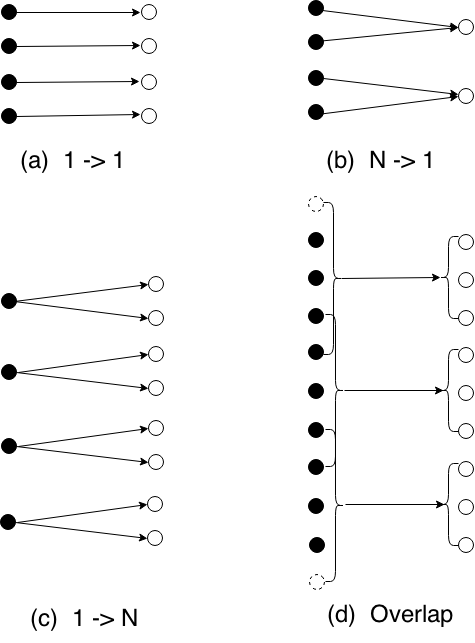
\includegraphics[scale=.50]{figures/template.png}
\caption{Relationship of Input and Output in Seismic Data Processing}
\label{Template}
\end{figure}
%%%%%%%%%%%%%%%%%%%%%%%%%%%%%%%%%%%%%%%%%%%%%%%%%%%%%%%

\section{Code Generator}

%After user created project and completed their own kernel codes, one component named Code Generator (CG) in SAC will generate complete Spark codes for running on Spark platform. The CG will parse configuration of user's project and generate Spark application outlined codes, merge them with user's codes. User could also upload existing source codes or libraries, all of which will be integrated into current working project managed by Simple Build Tool (SBT). CG will also generate compiling and running scripts basing on user's runtime setting. All these scripts will be called by the web interface, on which some other information such as compiling and running status, location of output will be shown clearly.

As explained in previous chapters, after generating a new project and finishing program by user, it is time to make it run. Code Generator (CG) in SAC will be in charge of such task: creating skeleton of project, generating template codes, setting up running time enviroments etc. Template was already discussed in previous secion, and the main issue is definition of input type and output type. With such information, CG could generate outline of function to be completed by user. Basing on user's configuration, CG will also generate backend codes for loading data sets to RDD and saving output RDD back to HDFS or database. SAC uses Simple Build Tool (SBT) \cite{ScalaSBT} and Ant \cite{ApacheAnt} as project management tools. To make such codes run on Spark, CG generate source files list and dependencies list for SBT, then SBT will build all source codes and generate .jar file for current project. CG will also generate all runtime libraries list for Ant, and Ant will package all libraries into one .jar file for executation on Spark. CG will generate compiling script and running script too, which will be called by web interface.


\section{Application Executation}

%In SAC, every user's project will be treated as one Spark application. CG will generate the main driver code for each project. Each application could be submitted to SAC for running after compiled successfully. At execution time, driver code will setup the Spark running time environment, call the SeismicVolume object to generate RDD and execute user's algorithms on top of RDD and then store the processed results on HDFS. It will clean up the running environment and release resources after finished. To make it support multiple users, Spark Jobserver \cite{SparkJobserver}  was introduced to this platform. Based on the priority of application and computation resources requirement of an application, an user could configure the running parameters: number of cores and memory size; and then submit his/her own job, monitoring job status and viewing the running results. Another big advantage of Spark Jobserver is supporting of NamedRDD that allows multiple applications share RDD but has only one copy cached in memory. For some complicate algorithms that need multiple steps or application running in workflow, NamedRDD is a good choice for boosting performance. After job is finished, the running results cloud be discarded or be saved to user's workspace basing on user's selection.

As PaaS cloud platform, SAC provides two ways of executing application: running one job on Spark and running multi-jobs with workflow on Spark. To process big seismic data, each job may take much time, so on such a multi-user platform, job submission and job scheduling need to be planned carefully. To start a job, user need to configure how much resource it needs (memory, number of cores, scheduling policy) at first, and then submit job to Spark-jobserver. Once the runtime environment is satisfied, the driver code call the SeismicVolume object to generate RDD and apply user's algorithms on RDD and then store the processed results on HDFS or database. If there are any tasks failure at running time, Spark will only run the failed tasks basing on dependencies chain. All job status could be checked through web interface of SAC, and after job is finished, user could view results imediately through visualization component. For the workflow including multiple widgets, it need a driver to setup DAG at first and each widget is a independent job with clear-cut input and output at running time, but they could share save Named RDDs with same context for boosting performnce.


\section{Application Programming Interface}
SAC itself is developed in Java/Scala language, so it could be compiled into jar library. User cloud call this library in his own application or use template and CG generate codes outline by filling algorithm snippet, but in both cases, user need to be familiar with API of SAC, configure application and control development procedure by himself. SAC also provides web interface to simplify installation of development environment on client side, in such case, user only need to select template, input codes snippet and then click buttons to compile, to run and to view results. 
When user want create a new algorithm or model, SAC will create a new project, in which user could select template, define data type of input and output, then SAC will generate function template for user to fill his own logic codes in it. SAC had integrated widely used libraries in seismic area such JTK, Breeze and OpenCV, so user could use them in programming or add his own libraries as requirement. After user finished coding, he could compile and run them immediately and view results after job finished. With web interface, user cloud also preview dataset, select data set as input for algorithm and check running result after job finished. Workflow is another big improvement for running batch jobs; Each long batch job are divided into small tasks, and each task is encapsulated as widget. User could select different widgets, configure parameter for each one and connect them into a long job, and then submit it to cluster. With workflow, the productivity, usability and flexibility are all improved. Currently, four main components on web interface: project coding and running, data set preview, job management and workflow. The web programs are written in PHP Language, JavaScript, HTML and CSS, while the workflow part are modified from Clowdflows \cite{ClowdflowsMain}. Some other popular web development components such as jquery, bootstrap, user cake, dropzone, D3 and ace editor are used in web interface. To make SAC framework be used by web interface, a bunch of shell scripts are developed and are called by web interface. XML files are used for communication between web interface and SAC framework. The example XML file used to describe project is shown as below. 

\lstset{language=XML,frame=single}
\begin{lstlisting}[float,caption=Sample XML file of Project Configuration,label=XMLProjectConfig]
<?xml version="1.0"?>
<ProjectConfig>
  <user>pvamucloud</user>
  <rootDir>/home/cscloud/user/pvamucloud/Pixel</rootDir>
  <projectName>Pixel</projectName>
  <projectVersion>1.0</projectVersion>
  <unit>Pixel</unit>
  <inputType>Float</inputType>
  <outputType>Float</outputType>
  <direction>Inline</direction>
</ProjectConfig>
\end{lstlisting}
